\label{ch:chapter02}
\gls{BTI} poses a significant challenge in ensuring the reliability of digital systems, affecting the delay of digital logic gates, which ultimately can lead into timing failures. Sophisticated defect-centric models have been developed and successfully calibrated against empirical data to forecast the impacts of \gls{BTI} at the device level. However, their application to large-scale digital circuits operating under realistic workloads over typical system lifetimes is limited because of the computational complexity of defect-centric models. To make the application of aging models in that context feasible, a useful technique is to compress the transistor workloads into simplified and hence manageable representative workloads. While fast in terms of execution speed, previous techniques struggle with accuracy when predicting aging degradation, and can reach a very high average error in threshold voltage increase prediction. In this work, we review the compression techniques described in the literature and propose two novel approaches that surpass existing ones in terms of accuracy, which is demonstrated for a complex digital design used as benchmark. Specifically, our best compression technique matches the predictions obtained through the reference uncompressed workloads, introducing negligible error, and maintains low execution times to efficiently and accurately scale defect-centric models to the circuit level.


\section{Introduction}
Among the aging phenomena affecting electronic devices, \gls{BTI} is of special significance due to its dominant impact on timing variability \cite{duchAnalysisFunctionalErrors2020, santana-andreoImpactBTIHCI2022, moritaEfficientAnalysisMitigation2022, klemmeEfficientLearningStrategies2022}. \gls{BTI} is driven by the gate biasing of the transistor, directly increasing its threshold voltage $(V_\text{th})$. This generally results in a longer propagation delay for logic gates, ultimately leading to potential timing violations. \gls{BTI} is widely attributed to the trapping and release of charge carriers from defects, which cause discrete stochastic shifts of the threshold voltage. To predict \gls{BTI} degradation, defect-centric models such as the Probabilistic Defect Occupancy (PDO) model \cite{martin-martinezProbabilisticDefectOccupancy2011} are employed. In these defect-centric models \cite{grasserParadigmShiftUnderstanding2011, reisingerUnderstandingModelingAC2011, kaczerDefectcentricPerspectiveDevice2015}, each defect has a certain mean carrier Capture and Emission Time (CET) and an induced threshold voltage shift $\eta$, whose values follow certain probability distributions. The number of defects in a transistor also follows a probability distribution. This inherent variability of \gls{BTI} results in a unique shift in threshold voltage for each transistor due to its unique set of defects. Defects with short CETs require just micro- to milliseconds of applied voltage (ON-time) to add their degradation to the transistor. However, defects with long CETs might require months of applied voltage to add their degradation. Similarly, when the applied voltage is removed (OFF-time), defects with short CETs will take less time to release their carrier and remove their degradation than defects with long CETs. Due to this wide spread of CET values, the actual activity/workload (ON/OFF phases during a transistor's lifetime) governs the induced threshold voltage due to BTI. 

The predictions obtained through the aforementioned physical models should closely match the experimental measurements \cite{saraza-canflancaDeterminationTimeConstant2022}, anticipating degradation at the end-of-life (EOL) of the circuit and providing designers with the ability to mitigate aging at design time. Due to the aforementioned nature of BTI, these predictions consist of aging variability distributions whose values are highly dependent on the transistor's bias conditions. Carrying this information from the device level to the circuit level without abstracting defects away (e.g., by modelling degradation or cell delay by empirical equations directly) is crucial to perform accurate degradation predictions \cite{vansantenModelingMitigatingTimeDependent2019}. However, the computation time required to directly solve the model equations taking into account realistic circuit workloads for each transistor (expressed in terms of a bias waveform $V(t)$ evolving over time) is unfeasible for large digital circuits \cite{vansantenDesigningGuardbandsInstantaneous2016} due to the need to recalculate the model parameters each time bias conditions change. Obtaining the degradation for a waveform with a frequency in the order of GHz at an EOL of 10 years requires an order of \num{e18} recalculations per transistor, an infeasible amount in computational cost. Different strategies have been reported in the literature to overcome this problem, focusing mainly on \textit{workload compression}, which revolves around reducing the complex, long waveform that represents the transistor's workload to a simpler waveform that retains enough information about the original signal to attain a comparatively close degradation to the one obtained through the original waveform. 
 

\textit{Our Novel Contributions are as Follows:}
\begin{enumerate}


    \item We review compression approaches employed in the literature, unifying the evaluation criteria and, for the first time, comparing these techniques with the same workloads on the same circuits for a fair comparison. These are judged under the same benchmark circuit on 7 nm FinFET standard cells from the open-source ASAP7 standard cell library \cite{vashishthaASAP7PredictiveDesign2017} in terms of speed and accuracy when predicting threshold voltage degradation and the subsequent change in delay, showing how the previous approaches in the literature have an unacceptably high error (73.34\% and 84.85\% average error in threshold voltage for the two approaches studied, when compared to the reference uncompressed workload). 
    \item We introduce and implement two novel compression approaches (\textit{Gate-level} and \textit{Super CDW}) to compress workloads with minimal accuracy loss (1.31\% and 2.31\% average error respectively, clearly surpassing the reviewed previous approaches) while achieving execution speeds sufficient for large digital circuits (1,151 and 146 seconds respectively, compared to 10 hours for the reference uncompressed workload, for a benchmark circuit with 3100 transistors).

   
\end{enumerate}

 % Together, these contributions will pave the way for computationally efficient aging simulations for digital circuits that fully take into account the complexity of underlying degradation phenomena. 
 
 %The paper is structured as follows: In Section \ref{section:ModelingBTI}, the equations that describe the defect-centric model are introduced. In Section \ref{section:RelatedWork}, the compression techniques used in the literature are reviewed. In Section \ref{section:Framework}, the framework used in this work is explained in detail, while in Section \ref{section:new_compression} the novel compression techniques introduced in this work are presented. In Section \ref{section:Results}, the performance of these techniques is evaluated against the ones presented in the literature, and finally, in Section \ref{section:Conclusions} conclusions are drawn. 

\section{Calculating BTI degradation with defect-centric models}
\label{section:ModelingBTI}
This section illustrates the calculation of the \gls{BTI} degradation caused by complex waveforms in a transistor, demonstrating the computational limitation when using uncompressed workloads in large digital circuits. In this work, the PDO model is employed \cite{martin-martinezProbabilisticDefectOccupancy2011}, which models the capture and emission of carriers in the defects of the gate dielectric of a transistor, being agnostic with respect to their physical properties. Defects are simply described in terms of three parameters (each depending on bias voltage and temperature): mean capture $\tau_c (\text{V},\text{T})$ and emission times $\tau_e (\text{V},\text{T})$ and the change on the transistor's threshold voltage $\eta (\text{V},\text{T})$. The mean capture and emission times represent, respectively, the average time it takes for a carrier to be captured by the defect when empty and for a carrier to be emitted when the defect is occupied. In this way, the emission probability $p_e$ given a certain time interval $\Delta t$ is $p_e=\Delta t / \tau_e$, while the capture probability is $p_c=\Delta t / \tau_c$. Time constants are modeled according to a bivariate lognormal distribution $D\left(\tau_e, \tau_c\right)$, as shown in Fig. \ref{fig:PDO_Intro}(a).
\begin{figure*}[!t]
    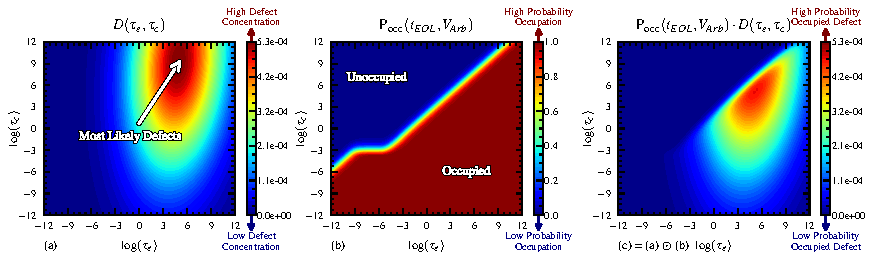
\includegraphics[width=\textwidth,trim={0 0.5mm 0 0mm},clip]{images/ch2/plot_pocc_ddefect_together.pdf}
    \caption{Representations in a logarithmic scale for the time constants of: (a) the distribution of defects used in this work; (b) the probability of a defect being occupied after an arbitrary waveform $V_{Arb}(t)$ with occupied and unoccupied defects highlighted; and (c) the product of both, which provides in the mean degradation through eq. (\ref{Equation:MeanVt}).}
    \label{fig:PDO_Intro}
\end{figure*}
Thus, any defect will have a certain probability of occupation ($\text{P}_{\text{occ}}$) that depends on the history of the operating conditions of the transistor, with a captured carrier adding its specific amplitude to the overall threshold voltage degradation value. Adding together the mean contribution of these defects, the mean degradation $(\overline{\Delta V_\text{th}})$ of a transistor at EOL ($t_\text{EOL}$) when compared to a fresh device (at $t_\text{fresh}$) can be obtained through the PDO model as:
\begin{equation}
\label{Equation:MeanVt}
\overline{\Delta V_{t h}}\left(t_\text{EOL}\right)=\bar{N} \bar{\eta} \iint_0^{\infty} D\left(\tau_e, \tau_c\right)  \Delta \text{P}_{\text{occ}}\left( t_\text{EOL}\right) \mathrm{d} \tau_e \mathrm{~d} \tau_c
\end{equation}
where $\bar{N}$ is the mean number of defects, $ \bar{\eta} $ is the mean change in threshold voltage for a single defect being charged and $\Delta \text{P}_{\text{occ}}\left(t_\text{EOL}\right)$ is the change in probability of occupation at EOL, defined as $\Delta \text{P}_{\text{occ}}\left( t_\text{EOL}\right) = \text{P}_{\text{occ}}\left(t_\text{EOL}\right) - \text{P}_{\text{occ}}\left(t_\text{fresh}\right)$. The value of $\text{P}_{\text{occ}}$ at any point in time depends on the time constants as well as on the biasing history of the transistor and can be expressed in differential form as a differential equation \cite{saraza-canflancaDeterminationTimeConstant2022} whose solution yields a general expression for the probability of occupation after a certain time interval $\Delta t =t_f - t_0$, under constant operating conditions (i.e., bias voltage and temperature) and given an initial value $\text{P}_{\text{occ}}(t_0)$ :
\begin{equation}
\label{Equation:Pocc}
\text{P}_{\text{occ}}(\Delta t)=\frac{\tau_e}{\tau_e+\tau_c}+\left(\text{P}_{\text{occ}}(t_0)-\frac{\tau_e}{\tau_e+\tau_c}\right) e^{-\left(\frac{1}{\tau_e}+\frac{1}{\tau_c}\right) \Delta t}
\end{equation}

An example of the resulting $\text{P}_{\text{occ}}$ from an arbitrary waveform is shown in Fig. \ref{fig:PDO_Intro}(b), as well as the product of this $\text{P}_{\text{occ}}$ with the distribution $D\left(\tau_e, \tau_c\right)$ in Fig. \ref{fig:PDO_Intro}(c), which after applying eq. (\ref{Equation:MeanVt}), results in the mean degradation of the transistor. 

Calculating the mean degradation at EOL requires knowing $\text{P}_{\text{occ}}(t_\text{EOL})$, which implies reevaluating eq. (\ref{Equation:Pocc}) for all CET values each time the operating conditions of the transistor change due to the dependence of ${\tau_e},{\tau_c}$ on temperature and voltage bias. The bias workload $V(t)$ for a transistor can use a \textit{Digital} format, i.e., with two discrete valid voltage values $V_{\text{high}}$ and $V_{\text{low}}$ or an \textit{Analog} format with continuous voltage values. The \textit{Digital} format is simpler, but some information is lost compared to the \textit{Analog} format, as in reality the voltage waveform is not perfectly square, with transition slopes, overshoots, and transient states due to the stacking effect \cite{HongStacking2007, firouziLinearProgrammingApproach2011}. Taking these effects into account has an impact on the resulting mean degradation, for example, not considering voltage overshoots results in an underestimation of 4 \% in degradation, as reported in \cite{gieringNBTIModelingAnalog2014}. 

Although the focus so far has been on obtaining the mean degradation and it will be used in this work as a metric to evaluate the accuracy of the aging prediction, one of the key features of a defect-centric model is the ability to model the aging variability of BTI. This can be done by considering, for each transistor, multiple sets of defects with their specific time constants and amplitude. Then, the contribution of these individual defects to the threshold voltage depending on their $\text{P}_{\text{occ}}$ is added together and multiple aging variability samples of $\Delta V_\text{th}({t_\text{EOL}})$ can be generated for the same transistor. This is crucial to analyze the effect of aging variability at the circuit level \cite{santana-andreoImpactBTIHCI2022,toro-friasFastAccurateReliability2015,vansantenModelingMitigatingTimeDependent2019}, which has been confirmed to have a significant effect on the performance of aged circuits \cite{santana-andreoReliabilityImprovementSRAM2024a, santana-andreoCharacterizingAgingDegradation2022, saraza-canflancaSmartSRAMCellArray2022}. To mitigate the effect of aging in digital circuits, a guardband (i.e., a timing slack on top of circuit delay) is typically used. When no aging variability information is available, a pessimistic, worst-case degradation is uniformly applied to all transistors. Meanwhile, in \cite{vansantenModelingMitigatingTimeDependent2019} it is shown how, by building aging variability-aware cell libraries, the required timing guardband is reduced by 46\%. Consequently, having the ability to consider the aging variability of \gls{BTI} (i.e., by not abstracting away the defects) is a critical feature of a methodology making aging predictions for large digital circuits. 

In any case, computing $\text{P}_{\text{occ}}(t_\text{EOL})$ considering the complete workload of each transistor until EOL is not feasible: considering a single transistor, an EOL of 10 years (around \num{3.15e+8} seconds) and a complex waveform with a mean frequency of around 4 GHz (in the order of the frequency of commercial processors \cite{AMDRyzenProcessors}) will require approximately \num{2.52e+18} iterations of eq. (\ref{Equation:Pocc}). This is a general problem for defect-centric models and not specific to the PDO model, as calculating the probability of occupation, which depends on the bias history of the transistor, to obtain the final degradation is a common element of defect-centric models \cite{grasserParadigmShiftUnderstanding2011, reisingerUnderstandingModelingAC2011, kaczerDefectcentricPerspectiveDevice2015}. To solve this issue, a naive approach is to assume that the transistor is at a constant, uniform high value (e.g., ignoring aging recovery entirely) so that eq. (\ref{Equation:Pocc}) is only computed once until EOL. However, this is not acceptable, as it significantly overestimates aging \cite{vansantenModelingMitigatingTimeDependent2019}. 
A better approach is to consider that the complex waveform that represents the transistor workload can be modeled as a shorter, representative periodic waveform of duration $\Delta t_{\text{signal}}$, such as the waveform corresponding to an application periodically triggered throughout the lifetime of the circuit. This imposes a limitation on the applications that can be considered, although they are typical in embedded systems \cite{amrouchConnectingPhysicalApplication2015} such as wireless body sensor networks \cite{duchAnalysisFunctionalErrors2020}, and for non-periodic applications the workload size can be adapted to make it more representative. Considering a period of total duration $\Delta t_\text{signal}$ consisting of $n$ total distinct points of bias $V_i$, each $i$-th point with their own $\tau_{ei}(V_i)$, $\tau_{ci}(V_i)$ and $\Delta t_i$ values, a general expression for $\text{P}_{\text{occ}}$ after $\Delta t_\text{signal}$ can be obtained by applying eq. (\ref{Equation:Pocc}) successively: 
% \begin{equation}
% \label{Equation:One_period}
% \text{P}_{\text{occ}}(t_0+ \Delta t_{\text{signal}})=A +B \text{P}_{\text{occ}}(t_0)
% \end{equation}
% where $A$ and $B$ are multiplicative factors:
% \begin{multline*}
% A=\sum_{i=1}^n \frac{\tau_{e i}}{\tau_{e i}+\tau_{c i}} \cdot\left(\prod_{j=0}^{n-i-1} e^{-\left(\frac{1}{\tau_{e(n-j)}}+\frac{1}{\tau_{c(n-j)}}\right)\Delta t_{(n-j)}}\right) \cdot
% \\\left(1-e^{-\left(\frac{1}{\tau_{e i}}+\frac{1}{\tau_{c i}}\right) \Delta t_i}\right) 
% \end{multline*}
\begin{equation}
\label{Equation:One_period}
\text{P}_{\text{occ}}(\Delta t_{\text{signal}})=A +B \text{P}_{\text{occ}}(t_0)
\end{equation}
where $A$ and $B$ are multiplicative factors. Factor $B$ is the weight of the initial probability of occupation on the final value, while $A$ is associated with the shift in probability of occupation due to the applied workload. As $\Delta t$ becomes larger, $A$ dominates over $B$ for more pairs of time constant values. They are defined as:

\begin{equation*}
f_k = e^{-\left(\frac{1}{\tau_{e k}}+\frac{1}{\tau_{c k}}\right) \Delta t_k} \ \ \ \  ; \ \ \ \ B=\prod_{i=1}^n f_i 
\end{equation*}
\begin{equation*}
A=\sum_{i=1}^n \frac{\tau_{e i}}{\tau_{e i}+\tau_{c i}} \cdot \left(1-f_{i}\right) \cdot\left(\prod_{j=0}^{n-i-1} f_{n-j}\right)  
\end{equation*}

Applying eq. (\ref{Equation:One_period}) over successive $M$ periods results in a geometric series, which can be expressed as:
\begin{equation}
\label{Equation:Pocc_periodic}
\text{P}_{\text{occ}}(M \Delta t_\text{signal})=A \frac{1-B^M}{1-B}+B^M \text{P}_{\text{occ}}(t_0)
\end{equation}
 This equation, applicable to any arbitrary periodic waveform \cite{gieringNBTIModelingAnalog2014}, reduces the number of evaluations of eq. (\ref{Equation:Pocc}) from each bias change until EOL to only changes in the considerably shorter representative waveform of duration $\Delta t_\text{signal}$ by considering $M=t_\text{EOL} / \Delta t_{\text{signal}} $. If, say, we assumed a 1 ms workload of an application execution to be representative of the operation until EOL, for the previous example of a mean frequency of 4 GHz the number of iterations of eq. (\ref{Equation:Pocc}) required to estimate degradation at EOL are significantly reduced from \num{2.52e+18} to \num{8e6}. Although the improvement is notable, reducing the number of iterations by 12 orders of magnitude, \num{8e6} iterations per transistor is still too large for a circuit with many transistors.  


\section{Related Work}
\label{section:RelatedWork}
Different approaches have been used to solve the issue of bringing workload-dependent aging predictions to large digital circuits. In \cite{klemmeMachineLearningCircuit2021,klemmeScalableMachineLearning2022a,klemmeEfficientLearningStrategies2022} the calculation of the probability of occupation is circumvented using a curve that translates the average duty cycle of the transistor workload directly into mean degradation, making the problem computationally trivial. Although the curve itself is obtained through a physics-based model \cite{thirunavukkarasuDeviceCircuitFramework2019}, the transistor-level information
$\text{P}_{\text{occ}}(t_0 + t_\text{EOL})$ required to model aging variability is lost in the process. Additionally, only average long-term degradation is obtained, so short-term degradation cannot be properly modeled. 

By contrast, the strategies in \cite{vansantenDesigningGuardbandsInstantaneous2016,AtomisticPseudoRodopoulos2014,fornaciariHarnessingPerformanceVariability2019, duchAnalysisFunctionalErrors2020, amrouchConnectingPhysicalApplication2015} focus on workload compression to obtain the degradation at EOL. Through compression, calculating $\text{P}_{\text{occ}}(t_\text{EOL})$ becomes computationally feasible, and the transistor-level information is not lost. In \cite{vansantenDesigningGuardbandsInstantaneous2016}, a compression technique was introduced that will be referred to as \textit{longest continuous stress (\textit{LCS}) compression}. By calculating the duty cycle $\lambda$ (ON-/OFF-ratio) and the longest continuous ON-time $t_{\text{LCS}}$, the original waveform is reduced to three points, a \textit{stress} phase where high voltage is applied for a time $t_{s}=\lambda t_\text{EOL}$, a recovery phase where low voltage is applied for $t_{r}=(1-\lambda) t_\text{EOL}$ and finally a LCS phase where high voltage is applied for $t_\text{LCS}$, as shown in Fig. \ref{fig:sect2waveformRepresentations}. The driving idea for this compression method is to use the first two phases to represent the average long-term impact of BTI, which is considered frequency independent, and the last LCS phase as a worst-case value of short-term BTI. This approach requires only three iterations of eq. (\ref{Equation:Pocc}) per transistor, significantly reducing the execution time.

\begin{figure}[!b]
    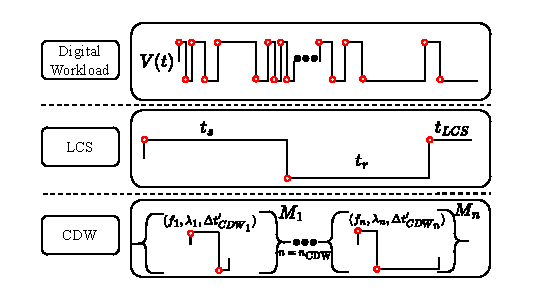
\includegraphics[width=0.48\textwidth,trim={7mm 3.5mm 10.5mm 3mm},clip]{images/ch2/WaveformRepresentationsSect2.pdf}
    \caption{Conceptual waveform representations for state-of-the-art compression techniques. For the \textit{LCS compression}, $t_s$ is the stress phase, $t_r$ the recovery phase and $t_{\text{LCS}}$ the longest continous ON-time in the original workload. For the \textit{CDW compression}, the duty cycle $\lambda$, frequency $f$, and total elapsed time $\Delta t'_{\text{CDW}}$ are the triplet of values that represent one workload segment and $M$ the number of times that segment is repeated. The number of data points, in red, drive the computational effort to obtain the transistor's degradation.}
    \label{fig:sect2waveformRepresentations}
\end{figure}

On the other hand, the authors in \cite{AtomisticPseudoRodopoulos2014} propose taking the uncompressed workload of duration $\Delta t_\text{signal}$, dividing it into segments, and simplifying them into \textit{Compact Digital Waveform} (CDW) segments. This method is termed \textit{CDW compression}, and is further utilized in \cite{duchAnalysisFunctionalErrors2020, fornaciariHarnessingPerformanceVariability2019}. A CDW segment consists on three values: duty cycle $\lambda$, average frequency $f$, and segment duration $\Delta t_{\text{CDW}}$. The values of each CDW segment match the average values of their corresponding original workload segment. In this way, a complex segment that, in the original workload, required many points to be described is reduced to a repeating two-point AC waveform with matching duty cycle and frequency. The number of periods $M$ for each segment is computed as $\Delta t_{\text{CDW}} \cdot f$. The CDW equivalent for the first and last segments of an example workload with their different triplet of values is shown in Fig. \ref{fig:sect2waveformRepresentations}. Thanks to this simplification, $\text{P}_{\text{occ}}$ can be computed significantly faster through eq. (\ref{Equation:Pocc_periodic}). The number of segments $n_\text{CDW}$ used to divide the workload is the user's choice, which introduces a trade-off between accuracy and computation time. Two options are possible when computing the CDW workload \cite{fornaciariHarnessingPerformanceVariability2019}: (a) to employ a fixed number of segments and divide the original workload into a number of intervals of certain, uniform duration $\Delta t_{\text{CDW}}$, or (b) to group segments with similar duty cycle $\lambda$ and average frequency $f$ through a dedicated algorithm.  Through this procedure, the degradation caused by one execution of the representative workload, after $\Delta t_\text{signal}$, can be easily calculated. Still, this degradation must be extrapolated to EOL, a much larger time value (e.g., years) than $\Delta t_\text{signal}$ (e.g., seconds). To perform this extrapolation, the authors in \cite{AtomisticPseudoRodopoulos2014} increase the $\Delta t_{\text{CDW}}$ value of each segment by a proportional factor to cover the entire time range, so that $(\sum{\Delta t'_{\text{CDW}}}) =  t_\text{EOL}$ \cite{AtomisticPseudoRodopoulos2014, fornaciariHarnessingPerformanceVariability2019}. However, this gives \textit{disproportionally more weight to the last CDW segments when determining the final degradation}, causing a prediction error.

 %An algorithm is also proposed as an alternative to group regions with similar CDW values together to improve the trade-off. 

Finally, there are works \cite{gholveCARATReliabilityAnalysis2023,vansantenBTIHCDDegradation2020,gensslerModelingPredictingTransistor2023, amrouchConnectingPhysicalApplication2015, duchAnalysisFunctionalErrors2020} where a ``short" initial aging simulation is performed, obtaining a degradation curve from which the degradation at EOL is extrapolated through a fitting procedure. Some of these fitting approaches employ compression \cite{amrouchConnectingPhysicalApplication2015, duchAnalysisFunctionalErrors2020} to be able to perform longer initial simulations and improve fit quality. However, this approach comes with fundamental drawbacks. By construction, these works abstract defects away, losing the transistor-level information required to accurately consider aging variability. Additionally, a fitting procedure is required for \textit{each individual transistor} in the circuit, adding significant computational and implementation overhead. Furthermore, the length required for the initial simulation to obtain a precise extrapolation is not clear (\qty{1}{\micro s} workload in \cite{gholveCARATReliabilityAnalysis2023,vansantenBTIHCDDegradation2020,gensslerModelingPredictingTransistor2023}, \qty{100}{s} workload in \cite{amrouchConnectingPhysicalApplication2015} and a \qty{10}{min} workload in \cite{duchAnalysisFunctionalErrors2020}) a so-called ``short" simulation can still include a high number of points. Due to these drawbacks, this work will only employ techniques to obtain degradation at EOL \textit{without abstracting defects away}, namely \textit{LCS compression} and the original \textit{CDW compression}. The two techniques proposed in this work (\textit{Gate-level} and \textit{Super CDW} compression, section \ref{section:new_compression}), satisfy this requirement with minimal accuracy loss. 

%Specifically, the works \cite{gholveCARATReliabilityAnalysis2023,vansantenBTIHCDDegradation2020,gensslerModelingPredictingTransistor2023} obtain the degradation curve after a \qty{1}{\micro s} workload. This degradation is extrapolated to EOL by using the easy-to-compute degradation from a DC stress to EOL as reference. In \cite{amrouchConnectingPhysicalApplication2015} the workload is divided into segments, compressing each one into a single two-point waveform that maintains the duty cycle of the original segment but disregards its frequency. Through this procedure, the degradation curve of a 100-s-long workload is obtained, to which the EOL extrapolation is applied. Lastly, in \cite{duchAnalysisFunctionalErrors2020}, they start from a 2 s workload, obtain the CDW-equivalent of that workload, and compute the degradation curve resulting from repeating those 2 s of activity for 10 minutes. Then, they extrapolate to EOL through a fitted curve and perform another short simulation adding the EOL degradation value to capture the short-term degradation.

\section{Reliability Framework}

\label{section:Framework}
In this section, the reliability framework employed in this work and its features are introduced. This framework needs to be able to, from a realistic, representative workload, extract its compressed counterparts and compare the degradation obtained through them with the one obtained without compression.

\subsection{CASE: A circuit-level aging simulator}

To evaluate the aging degradation of each digital gate, we employ our circuit-level aging simulator, CASE \cite{martin-lloretCASEReliabilitySimulation2017}. CASE works with a certain circuit netlist as input, simulates the circuit topology with the SPICE circuit simulator taking into account aging variability and returns the aging-induced degradation per transistor and the circuit's aged performances. This is necessary as current commercial tools such as RelXpert \cite{CadenceReliability} or PrimeSim MOSRA \cite{SynopsysReliability} employ deterministic compact models, unable to accurately model aging variability when compared to defect-centric models. To estimate the impact of aging on digital circuit delays, it is important to work at the transistor level, since not taking individual transistor degradations into account will result in erroneous estimations \cite{khanBTIImpactLogical2012, vansantenModelingMitigatingTimeDependent2019, vansantenNewWorstcaseTiming2019}, with degradation on certain transistors having a larger impact on circuit delay and therefore being more susceptible to aging \cite{mohamedGraphAttentionNetworks2024}. CASE was conceived to study the circuit degradation at the electrical level, obtaining the workload of each transistor through SPICE simulations by specifying a transient simulation. Additional features were required for this work, such as a module to compute the probability of occupation through an efficient implementation of eq. (\ref{Equation:Pocc_periodic}) and the ability to work with workloads expressed in different formats, as detailed in the next subsection. 

%When employing an analog format, a set of gate inputs is specified in a SPICE standard VEC digital vector file format, a transient simulation is performed, and the transistor's workload is obtained. For the digital format, the individual workloads of each transistor are fed directly into the simulator's aging calculation through an external file, bypassing the need to perform electrical simulations in SPICE.


% Given how the number of iterations of (\ref{Equation:Pocc}) is determined by the number of transient points used to describe these analog waveforms, it is important to reduce the number of points employed to describe it to the minimum required. This is distinct from compression, as it refers only to optimizing the workload waveform without changing its shape. For an analog representation, the waveform is represented by evenly spaced points in the time domain printed by the electrical simulator, even if there is no significant voltage change between two points, which is the case for most of the period of a transistor workload in a digital gate. To remove these redundant points, sections of similar voltage values, i.e., where points are within a certain range from the first point of the section, are grouped together. In this work a value of 10 mV is used as the maximum distance between points for each group. However, digital workloads do not require any post-processing, as there are only two possible voltage values. In that case,

% \subsection{Probability of occupation at time zero}
% To apply eq. \ref{Equation:Pocc}, a value for $\text{P}_{\text{occ}}(t_0)$ at time zero is required. Applying that equation for a situation where the device is left unbiased indefinitely $(V = 0, \Delta t = \infty)$, a reasonable assumption for a fresh, unused device, results in a certain, non-zero probability of occupation $\text{P}_{\text{occ}}(t_{0})$ as shown in Fig. \ref{fig:IntialPocc}. One may consider that probability at the begining of the lifetime of a device to be zero, but that would result in a number of defects being occupied on the first application of (\ref{Equation:Pocc}) and a significant mean degradation even after an infinitesimally small $\Delta t$. To correct for the resulting offset, probability of occupation is redefined as:
% \begin{equation}
% \label{Equation:Pocc_adjusted}
% \Delta \text{P}_{\text{occ}}(\Delta t)=\text{P}_{\text{occ}}(\Delta t) - \text{P}_{\text{occ}}(t_0)
% \end{equation}
% Which, for the arbitrary waveform employed in Fig. \ref{fig:PDO_Intro} (b) results in the probability of occupation shown in Fig. \ref{fig:IntialPocc} (b).
% \begin{figure*}[!t]
%     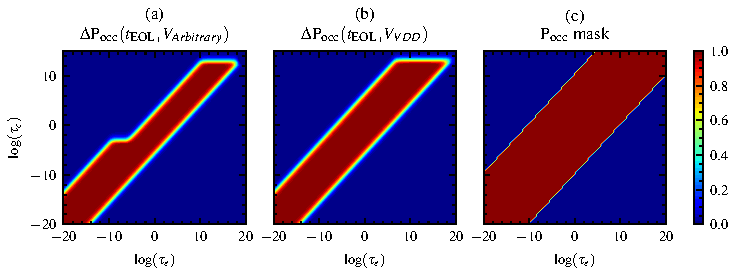
\includegraphics[width=\textwidth,trim={-5mm 0.5mm -5mm 0mm}]{images/ch2/plot_together_pocc.pdf}
%     \caption{Increase in probability of occupation due to the application until EOL of (a) the arbitrary waveform employed in Fig. \ref{fig:PDO_Intro} and (b) the worst-case probability of occupation after constant DC stress. In (c), the mask extracted from (b) of relevant values to calculate with a tolerance of $10^{-6}$, which reduces the computational effort to obtain the probability of occupation without impacting the precision of the degradation prediction.}
%     \label{fig:IntialPocc}
% \end{figure*}
% \subsection{Probability of occupation masking}

% As already mentioned, calculating $\Delta P_{\text{occ}}$ is the critical aspect in terms of execution time to obtain the degradation at EOL. Taking, for example, the arbitrary waveform used to obtain Fig. \ref{fig:PDO_Intro} (b), the change $\Delta P_{\text{occ}}$ is shown in Fig. \ref{fig:IntialPocc} (a).
% To reduce the computational effort to calculate $\Delta\text{P}_{\text{occ}}$ to a minimum, one can determine the region of CET values that is relevant for \gls{BTI} degradation, so that only the values contained in that area are re-evaluated. A high bound for degradation, considering the gate bias dependence, is a situation in which the transistor remains biased at a high voltage until EOL, equivalent to a constant DC stress. The evaluation of the degradation in this case is trivial, as it requires only one application of (\ref{Equation:Pocc}). The resulting $\text{P}_{\text{occ}}$ is shown in Fig. \ref{fig:IntialPocc} (b). Then, we can define a certain tolerance beyond which the change in the probability of occupation is considered to be zero and not recalculated each time. The mask generated from this approach is shown in Fig. \ref{fig:IntialPocc} (c) and significantly reduces the number of values that must be computed, resulting in an improvement of the execution speed.


\begin{figure}[!b]
    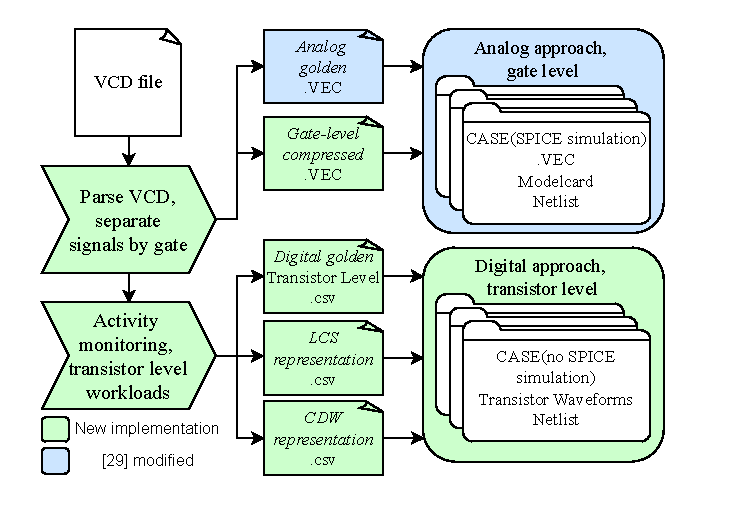
\includegraphics[width=0.48\textwidth,trim={7mm 3.5mm 13mm 4.5mm},clip]{images/ch2/FrameworkCellweaver.pdf}
    \caption{Overview of the flow employed in this work to analyze different compression approaches.}
    \label{fig:Framework Diagram}
\end{figure}
\subsection{Extending CASE to large digital circuits}
\label{ss:ExtendingCASE}
 A custom script is employed to implement the flow illustrated in Fig. \ref{fig:Framework Diagram}, building a reliability framework to extend CASE from small circuits like individual cells to large scale circuits with thousands of cells. First, to obtain the input vectors of each digital cell, a gate-level HDL simulation is performed on the circuit under study, resulting in a standard \textit{Value Change Dump} (VCD) file with input vectors (i.e., cell inputs) expressed in terms of logic levels, that is, $V_{\text{high}}$ or $V_{\text{low}}$ voltage levels. Input vectors are usually automatically translated into individual transistor level waveforms through the SPICE-level transistor topology from the standard cell library from the Process Design Kit (PDK) \cite{vansantenDesigningGuardbandsInstantaneous2016, duchAnalysisFunctionalErrors2020, fornaciariHarnessingPerformanceVariability2019}, in what is referred to as \textit{Activity Monitoring}. This results in a digital format workload of each transistor, which can be fed directly into the aging simulation through an external file without performing SPICE simulations, as shown in the bottom half of Fig. \ref{fig:Framework Diagram}. However, a reduction to a square-wave signal with only two possible logic values purposely removes information (e.g., rise time, transient states in intermediate nodes) potentially altering the predicted aging-induced degradation, particularly in complex cells with many transistors. For example, for two serially connected transistors, the intermediate node can be in an indeterminate state when both transistors are OFF. This state depends on the previous logic state and the charge leakage of that node \cite{zhangAgingAwareGateLevelModeling2021}, a level of detail which cannot be captured by \textit{Activity Monitoring}. An alternative to avoid this is to specify the input vectors in a SPICE standard VEC digital vector file format, perform a transient simulation, and obtain the transistor’s analog format workload. To compare both approaches, we name the uncompressed analog waveform as \textit{Analog Golden} and the uncompressed digital waveform as \textit{Digital Golden}. Later we will introduce other analog/digital compressions and use the golden references as the baseline. Although accurate, these workloads require long execution times that are \textit{unbounded}, i.e., they will require more time for longer workloads.

\subsection{Strategy for low frequency workloads}


\label{subsection:Defect_distribution_shifting}

Performing the aging simulations for a workload corresponding to low switching frequencies introduces an issue, as simulation has to cover at least one full period (which gets longer at the lower frequency) of the representative workload. Unfortunately, the switching frequency is much lower than the clock frequency in a circuit. For instance, an Adder which solely adds small numbers will keep its most significant bit at ``0''. Therefore, the switching frequency $f_\text{switch}$ of a transistor is typically much lower than the clock frequency $f_\text{clk}$ of a circuit. The work in \cite{vansantenWorkloadDependenceSelfHeating2020} showed how in a processor with a 2-GHz $f_\text{clk}$, $f_\text{switch}$ is actually in the kHz-range. These kHz frequencies are currently not supported due to how slower workloads will require more simulation time. An example is shown in Table \ref{tab:lowfreqexample}, where the degradation of an inverter is calculated using the \textit{Analog Golden} approach. It is clear how the simulation time and resulting VEC file size grow linearly with the reduction in frequency, making detailed simulations for slower signals unfeasible. Changing the frequency of the input signal without changing the workload duration is not an acceptable solution either, as it will distort the workload of each transistor.

\begin{table}[!t]
    \caption{Computational effort for low frequency workloads}
    \begin{center}
    \addtolength{\tabcolsep}{-0.2em}
       \begin{tabular}{@{}lcccc@{}}\toprule
        & \multicolumn{3}{c}{Frequency} \\   \cmidrule(lr){2-5}
                        & 500 MHz  & 50 MHz & 5 MHz & $<$1 MHz\\ \midrule
        Waveform Length & \qty{1}{\micro s} & \qty{10}{\micro s} & \qty{100}{\micro s} & Unfeasible \\
        Waveform File Size & 10 MB & 100 MB & 1 GB & Unfeasible\\
        Execution time  & 10 s & 30 s & \makecell{Memory error} & Unfeasible  \\ \bottomrule
    \end{tabular}     
    \end{center}
    \label{tab:lowfreqexample}
\end{table} 

A useful strategy to solve this problem is to keep the workload at a high frequency and instead scale the distribution of defects, changing its time constants to match the reduction in circuit frequency. In this way, only the PDO parameters have to be changed, bypassing the need to change the simulated workload and the slower execution times for slower workloads. \textit{It is important to note that these two approaches are mathematically equivalent and thus result in exactly the same result (no accuracy loss).} This equivalence is proven as follows: we start with a certain \textit{frequency factor} $\epsilon$, which determines how much the workload is slowed down and plug it in eq. (\ref{Equation:Pocc}). If we consider a certain slower workload, $\Delta t$ is increased so that the new $\Delta t' = \epsilon \Delta t$. The technique used is to keep $\Delta t$ unchanged and instead modify the time constants so that $\tau_e', \tau_c' = \tau_e / \epsilon , \tau_c / \epsilon$. Plugging these time constants into eq. (\ref{Equation:Pocc}) results in the \textit{same probability of occupation as the one obtained with the longer $\Delta t$.} The shift in the defect distribution means that we also have to shift the simulation time ($t_\text{EOL}$) in the opposite direction to ensure equivalency when extrapolating through eq. (\ref{Equation:Pocc_periodic}), so that $t'_\text{EOL} = t_\text{EOL} / \epsilon$. 


\section{Proposed compression methods}
\label{section:new_compression}
In this section, we propose two novel compression methods, \textit{Gate-level compression} and \textit{Super CDW compression}.

\subsection{Gate-level compression}
Since the compression methods found in the literature are used only for digital formats of the transistor $V(t)$ waveform, an alternative method is proposed for analog formats. This method is termed \textit{Gate-level compression}. Instead of compressing transistor waveforms, our method compresses the cell's input vectors. For example, consider a 2-input gate with inputs A, B and for which the four possible input vectors are (A = 0, B = 0), (A = 1, B = 0), (A = 0, B = 1), (A = 1, B = 1). The occurrence of each input vector and how frequently they change is recorded for a representative period. We then create a set of synthetic compressed input vectors with each combination appearing only once and maintaining the occurrence ratio of each combination, as shown in Fig. \ref{fig:GateLevelCompression}. The gate is simulated in SPICE for the compressed VEC file generated (as shown in Fig. \ref{fig:Framework Diagram}), extracting the individual transistor waveforms $V(t)$ in analog format. Compared to the methods found in the literature, using this format has the advantage of enabling multiple transistor bias values, while keeping the execution time bounded. This will result in more accurate results as the real bias conditions of the cell are considered (with slopes, overshoots...) and it can be useful in situations where the circuit operates at different supply voltages; for example, a digital circuit that operates between low-power mode ($V_\text{DD}= \qty{0.7}{V}$) and high-performance mode ($V_\text{DD}=\qty{1.0}{V}$) and switches between these two voltages. The drawbacks are requiring more points than a digital signal and performing SPICE calls for short simulations, as well as the inability to properly model short-term BTI, which will come to light in subsection \ref{subsection:freq_dependence}. 

\begin{figure}[!t]
\captionsetup{labelfont={color=blue}}
    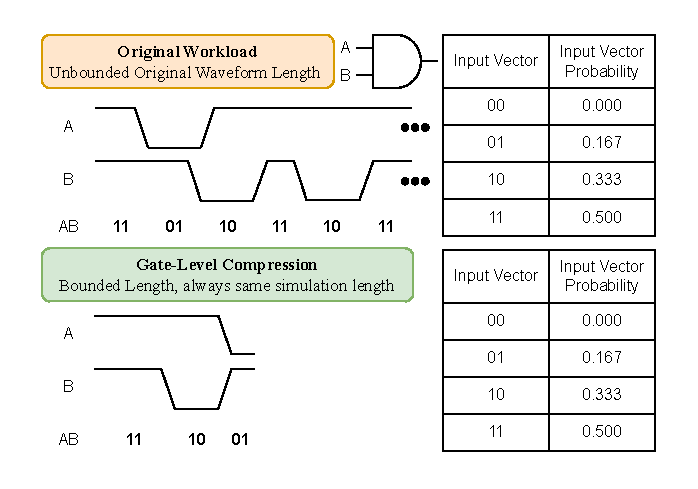
\includegraphics[width=0.48\textwidth,trim={7mm 5mm 7mm 6mm},clip]{images/ch2/GateLevelCompression.pdf}
    \caption{Example showing how \textit{Gate-level} compression is performed on a 2-input AND gate for one period of the representative waveform. }
    \label{fig:GateLevelCompression}
\end{figure}


\subsection{Super CDW compression}
\label{subsection:SuperCDWcompression}
Although the \textit{CDW compression} technique is quite efficient, performing the extrapolation to EOL by increasing the $\Delta t_{\text{CDW}}$ of each segment is a weakness, as it will give significantly more weight to the last CDW segments, resulting in an erroneous prediction. To avoid this weakness, we propose a technique termed \textit{Super CDW compression}. Each waveform is first translated to a set of CDW segments, as in the original \textit{CDW compression}. Then, instead of modifying $\Delta t_{\text{CDW}}$, we repeat the process used to derive eq. (\ref{Equation:Pocc_periodic}), obtaining the degradation after $M_{\text{super}}$ successive sets of CDW segments. Each CDW segment $k$ has its corresponding values $A_k$ and $B_k$, obtained by the expressions in eq. (\ref{Equation:One_period}). Applying a complete set of these segments for a number of segments $n_{\text{CDW}}$ will result in the following expression according to eq. (\ref{Equation:Pocc_periodic}):

\begin{equation}
\label{Equation:Super_CDW}
\text{P}_{\text{occ}}(\Delta t_{\text{signal}})=A_{\text{super}} +B_{\text{super}} \text{P}_{\text{occ}}(t_0)
\end{equation}
with:
\begin{equation*}
A_{\text{super}}=\sum_{k=1}^{n_{\text{CDW}}} A_k \frac{1-B_k^{M_k}}{1-B_k} \cdot\left(\prod_{l=0}^{n_{\text{CDW}}-k-1} B_{n_{\text{CDW}}-l}^{M_k}\right)  
\end{equation*}

\begin{equation*}
B_{\text{super}}=\prod_{k=0}^{n_{\text{CDW}}} B_k^{M_k}
\end{equation*}
In the same way as before, applying eq. (\ref{Equation:Super_CDW}) over successive $M_{\text{super}}$ periods results in a geometric series, which can be expressed as:
\begin{equation}
\label{Equation:Super_CDW_periodic}
\text{P}_{\text{occ}}(M_{\text{super}} \Delta t_\text{signal})=A_{\text{super}} \frac{1-B_{\text{super}}^{M_{\text{super}}}}{1-B_{\text{super}}}+B_{\text{super}}^{M_{\text{super}}} \text{P}_{\text{occ}}(t_0)
\end{equation}


Consequently, we have $M_k = \Delta {t_{\text{CDW}}}_k / f_k$ for each individual segment $k$ and $M_{\text{super}} = \Delta t_\text{signal} /  t_\text{EOL}$ for the collection of segments to reach EOL. Unlike \cite{AtomisticPseudoRodopoulos2014}, our approach repeats the same complete periodic waveform $M_{\text{super}}$ times instead of distorting the CDW segments to match $ t_\text{EOL}$ and applying only the periodic waveform once. An example showing how a CDW segment is extrapolated with our \textit{Super CDW} technique and the original \textit{CDW} approach in \cite{AtomisticPseudoRodopoulos2014} is shown in Fig. \ref{fig:CDWvsSuperCDW}. The \textit{CDW} method increases the $\Delta t_{\text{CDW}}$ of each segment to reach EOL, which results in a distorted workload, where, in the example shown in the figure, a part of the workload that would only last for 10 ms lasts for 1 year. The \textit{Super CDW} compression avoids this issue by performing the extrapolation in two steps, one for the duration of the segment compared to the workload and another for the entire workload. 

\begin{figure}[!t]
    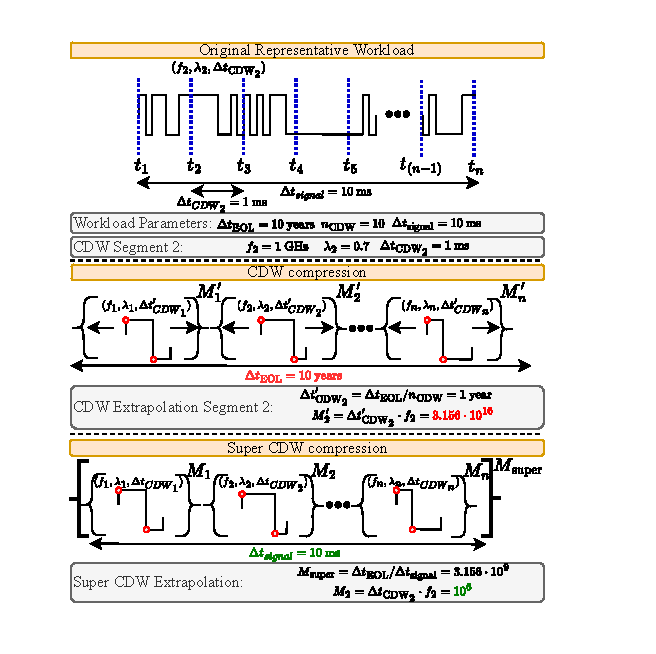
\includegraphics[width=0.48\textwidth,trim={11mm 8mm 18.5mm 5mm},clip]{images/ch2/CDWvsSuperCDW.pdf}
    \caption{Example showing how waveforms are extrapolated to EOL for the \textit{CDW} method \cite{AtomisticPseudoRodopoulos2014} and the \textit{Super CDW} method presented in this work. In this example, the third CDW segment representing 1 ms of an arbitrary workload is used to illustrate the differences between both methods. }
    \label{fig:CDWvsSuperCDW}
\end{figure}

The \textit{CDW} method requires a user-driven trade-off in the number of segments employed. This governs the (super) CDW fidelity/resolution and is a trade-off in accuracy versus computational effort. For instance, we can consider an inverter comprising a PMOS and an NMOS transistor whose input signal has two regions, split in the middle, of complementary signal probability, e.g., $\text{SP } (0.8 = 80\% )$ and $1-\text{SP } (0.2 = 20\%)$, as shown in Fig. \ref{fig:CDWTestPoints}. The length of the signal is set at 10 ms, while the frequency is set at 2 MHz and the degradation is calculated at an EOL of 10 years. The NMOS duty cycle is equal to the signal probability $\lambda_{\text{NMOS}} = \text{SP}$, while the PMOS duty cycle is $\lambda_{\text{PMOS}} = 1 - \text{SP}$. From start to finish the signal in Fig. 6 has a duty cycle of 0.5, however, smaller regions within might temporarily exhibit different duty cycles (shown 0.2 and 0.8 in the signal halves in Fig. \ref{fig:CDWTestPoints}). In fact, if we set $n_\text{CDW}$ to 1, we end up with an overall duty cycle of 0.5 as the later half of the signal averages out with the first half. However, starting from $n_\text{CDW} \geq 2$, we can correctly represent the duty cycle with 0.2 and 0.8 respectively (see Fig. \ref{fig:CDWTestPoints}). Comparing the degradation obtained for two segments for different values of $\text{SP}$ will give an insight into the potential error by oversimplifying the signal. Hence, we can represent the error range as a function of the heterogeneity of the input signal, since the one-segment workload will always predict the same degradation. The difference comes from the finer resolution of the \textit{CDW} method at $n_\text{CDW} > 1$. These temporarily higher or lower duty cycles are taken into account when $n_\text{CDW} > 1$ and might stimulate short-term BTI, i.e., have an impact on the final degradation. Furthermore, the final BTI-induced $\Delta V_{th}$-value differs considerably if the transistor ends under stress (high degradation) or with recovery (low degradation). Since CDW does not determine ending on 0 (OFF = recovery) or 1 (ON = stress), we explore this with the following test: we will consider the difference in the resulting degradation when the last segment is arbitrarily set at high or low and when it is set to finish at the same value as the original signal, i.e., with a matching end state. Exploring the error by setting $n_\text{CDW}$ to 1 (oversimplifying) and 2 (considering temporary differences in each half) is shown in Fig. \ref{fig:CDWTestFinishSweep} (a). We can observe that if the difference between the halves is more extreme (drifting further away from the overall average of 0.5), the importance of using the appropriate number of CDW segments increases. Actual signals might require $n_\text{CDW}$ at values higher than 2, which will increase with the heterogeneity of the uncompressed workload. Using the matching end-state approach results in the best-case error in each case, particularly for these extreme values. Consequently, it will be the approach used moving forward.


\begin{figure}[!t]
    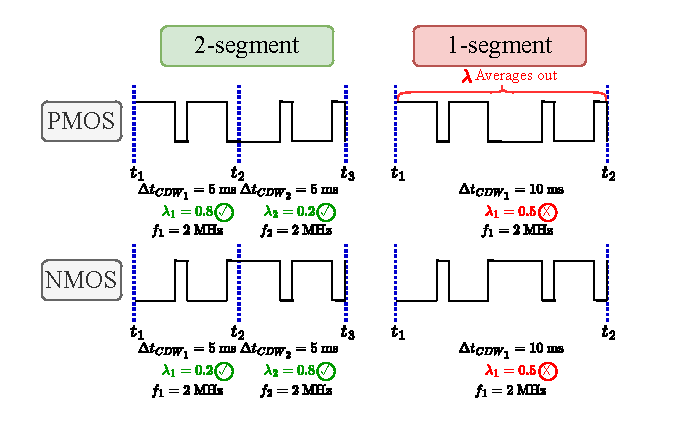
\includegraphics[width=0.48\textwidth,trim={7mm 5mm 13mm 3mm},clip]{images/ch2/CDWTestPoints.pdf}
    \caption{Conceptual representation of the waveforms employed to illustrate the accuracy vs. number of segments trade-off.}
    \label{fig:CDWTestPoints}
\end{figure}
\begin{figure*}[!t]
    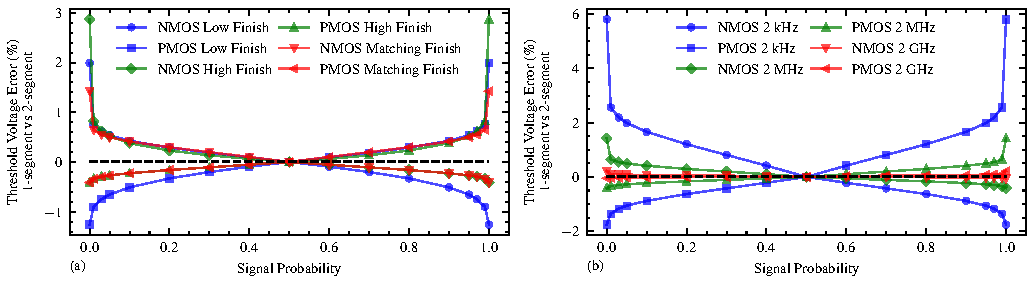
\includegraphics[width=\textwidth,trim={0 0 0 0},clip]{images/ch2/joint_plot_vth_difference_sign_finish.pdf}
    \caption{Error in computing the threshold voltage when comparing the 1-segment to the 2-segment workload as a function of signal probability, with different: (a) finishing values and (b) frequencies.}
    \label{fig:CDWTestFinishSweep}
\end{figure*}


Another aspect that influences this error is the total duration of each segment $\Delta t_{\text{CDW}}$. Depending on the strength of short-term and long-term \gls{BTI} the error introduced by ignoring the temporarily higher/lower SP becomes higher or lower. This is governed by the switching frequency. To prove this, we repeat the test varying the frequency, as shown in Fig. \ref{fig:CDWTestFinishSweep} (b). We consider 2 GHz, 2 MHz and 2 kHz. The results clearly show how the error increases significantly when considering the slower case, while it is reduced when considering the faster case. Given how the frequency of the signal will determine the significance of the short-term component of BTI, the compression methods used in this work will be tested under different frequencies to ensure they are universally applicable for a wide range of workload frequencies. 




\section{Results and discussion}
\label{section:Results}

In this work, a 32-bit Multiply-and-Accumulate (MAC) unit (a typical computing block in DSPs or in artificial intelligence accelerators such as systolic arrays or tensor processors) is synthesized and used as a benchmark circuit. This block multiplies an 8-bit weight by an 8-bit value and accumulates the result with a 32-bit partial sum. The block contains a total of 459 logic gates, comprising 3,100 transistors. Two workloads are considered for this circuit with the goal of obtaining the degradation after 10 years of operation. For workload ``W1'', we consider $f_\text{clk} = \qty{100}{MHz}$ and inputs (value, weight) follow a uniform random distribution and update every $\qty{10}{ns}$ for a total duration of $\qty{10}{\micro s}$, making it an unbiased, fair workload. This results in an output where the first 16 least significant bits are frequently switching, while the next ones only switch when enough multiplications have been accumulated, as illustrated in Fig. \ref{fig:MAC_bit_dist}. In fact, inspecting the distribution of values, the 16 least significant bits are constantly changing as they are the product of two random numbers. The next bits accumulate the result of the products, so they have a decreasingly low switching frequency. The last bits are zero, as not enough products have been performed to fill the output register. As a result, a wide range of patterns emerge, which will reflect in the internal gate workloads, clearly showing how a certain frequency for the input signal translates into different switching frequencies for the transistors depending on the location within the circuit's netlist. A second workload ``W2'' is considered. It is identical to the previous one for the initial $\qty{8}{\micro s}$ of simulation, but diverges in the final $\qty{2}{\micro s}$, during which all inputs are set to zero and the reset is activated. This represents sleep periods in circuits that, in many applications, are not active during their entire lifetime \cite{duchAnalysisFunctionalErrors2020}. The workload W2 is equivalent to the distribution in Fig. \ref{fig:MAC_bit_dist} for the first 800 product operations and has 0 in all output bits for the remaining 200. While other non-uniform workload scenarios exist, these two serve as unbiased benchmarks: one fully random and the other with a sharp inhomogeneity, facilitating a clear analysis of compression approaches. Simulations are performed with the open-source ASAP7 7nm PDK \cite{vashishthaASAP7PredictiveDesign2017}.
\begin{figure}[!t]
    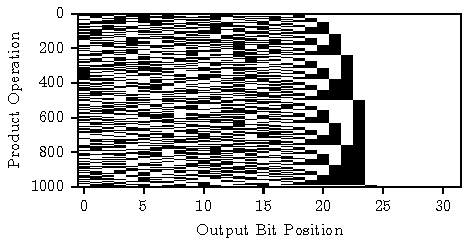
\includegraphics{images/ch2/MAC_bit_distribution.pdf}
    \caption{Output bit value distribution for the first MAC unit testbench, with 0s in white and 1s in black. }
    \label{fig:MAC_bit_dist}
\end{figure}
%with aging parameters extrapolated from experimental measurements \cite{saraza-canflancaDeterminationTimeConstant2022, saraza-canflancaStatisticalCharacterizationTimeDependent2021a}. 
Although the results reported here have been developed for this technology, the methodology is applicable for any technology in which \gls{BTI} can be properly modeled using individual charge trapping-detrapping events, spanning bulk CMOS (45nm and 65nm in \cite{procelDefectCentricPerspectiveChannel2015} or 28nm in \cite{kaczerDefectcentricPerspectiveDevice2015}), FinFET (8nm and 7nm in \cite{jiangTimeDependentVariability2021a}), Gate-All-Around (GAA) Nanosheet FETs \cite{choudhuryAnalysisBTISHE2020} and stacked Nanowire GAA FETs \cite{chasinBTIReliabilityTimedependent2017}. 

Seven different approaches to obtain the degradation of the MAC unit are considered: two used as reference for accuracy (\textit{Analog Golden}, \textit{Digital Golden}), two from the state-of-the-art  (\textit{5-segment CDW},  \textit{LCS}), two introduced in this work (\textit{Gate-level}, \textit{5-segment Super CDW}) and a baseline \textit{1-segment CDW}. The \textit{1-segment CDW} approach compresses the entire workload into one segment, being the coarsest and fastest implementation of the \textit{CDW} method for which both the \textit{Super CDW} approach proposed in this work and the \textit{CDW} approach in \cite{AtomisticPseudoRodopoulos2014} are mathematically equivalent. However, this represent the crudest approximation of the workload and additional segments are required to obtain higher accuracy in the degradation predictions for non-uniform workloads \cite{AtomisticPseudoRodopoulos2014}. A fixed number of segments is used to compute the \textit{5-segment CDW} and \textit{5-segment Super CDW} workloads, resulting in five segments of equal length. Five segments are the minimum required to properly model the hetereogeneity of the ``W2'' workload, so that the sleep period is included in a single segment. A diagram presenting the workload representation for each approach is shown in Fig. \ref{fig:sect4waveformRepresentations}. For \textit{LCS} and \textit{CDW} the representations were shown in Fig. \ref{fig:sect2waveformRepresentations}. Furthermore, Table \ref{tab:approaches} summarizes the main characteristics of each approach. They are evaluated below in terms of their required computational effort and their ability to predict threshold voltage degradation, analyzing finally how these differences in threshold voltage prediction impact the delay of the digital gates in the circuit.
\begin{figure}[!t]
    
    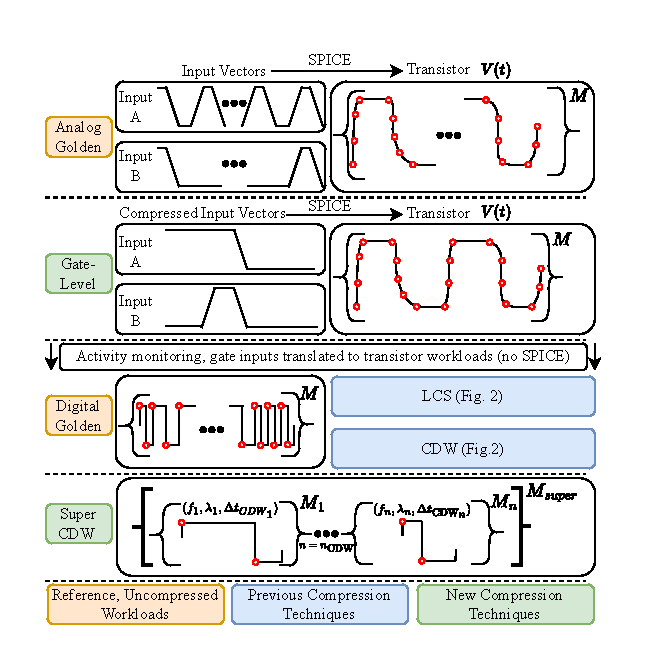
\includegraphics[width=0.48\textwidth,trim={7.5mm 6mm 10mm 8mm},clip]{images/ch2/WaveformRepresentationsSect4.pdf}
    \caption{Conceptual workload representations for the approaches under analysis. Golden workloads are unbounded (will increase in size with larger workloads). }
    \label{fig:sect4waveformRepresentations}
\end{figure}

\begin{table}
    \caption{Compressed and Uncompressed approaches used in this work}
    \begin{center}
    \addtolength{\tabcolsep}{-0.2em}
       \begin{tabular}{@{}lccc@{}}\toprule
        Approach & \makecell{Workload \\ format} & \makecell{ SPICE \\ required} & Eq. (\ref{Equation:Pocc}) iterations \\ \midrule
        \textit{Analog Golden} [Reference] & Analog & Yes & Unbounded (Very high) \\
        \textit{Digital Golden} [Reference] & Digital & No & Unbounded (High) \\
        \textit{Gate-level} [Our work] & Analog & Yes & Bounded (Low)  \\
        \textit{LCS} \cite{vansantenDesigningGuardbandsInstantaneous2016} & Digital & No &  3 \\
        \textit{1-seg. CDW} \cite{AtomisticPseudoRodopoulos2014} & Digital & No &  2 \\
        \textit{5-seg. CDW} \cite{AtomisticPseudoRodopoulos2014} & Digital & No &  10 \\
        \textit{5-seg. Super CDW} [Our work] & Digital & No &  10 \\ \bottomrule
    \end{tabular}     
    \end{center}
    \label{tab:approaches}
\end{table} 

\subsection{Execution speed}
The reduction in execution time through compression is shown in Fig. \ref{fig:Execution time} for workload W1. We plot the execution time of each circuit (cell) versus the number of transistors within the cell to indicate that larger circuits require longer times. Both golden simulations are unbounded and hence impose limits on the maximum circuit/workload size still feasible to simulate. The \textit{Gate-level} approach, although bounded, is considerably slower than the other compressed methods, which do not use an analog representation or require SPICE executions. The compressed methods using a digital format can handle larger circuits in computation times below 1 second. The total computation time of the 1-segment approach is lower by 1.27X when compared to the 5-segment. Execution times are strongly correlated with the number of iterations of eq. \ref{Equation:Pocc} required, as can be seen in Table \ref{tab:approaches}. Note that workloads compressed through the \textit{LCS}, \textit{CDW} and \textit{Super CDW} compression methods have their number of points (and thus, iterations) set to a specific value by construction. The number of iterations in the golden approaches is unbounded because the longer the workload duration, the higher the number of points. The number of iterations of the \textit{Gate-level} approach is bounded because independently of the workload duration, the number of input vectors of each cell is necessarily limited. Except for very short workloads, this number will be considerably smaller than for the golden approaches.

\begin{figure}[!t]
    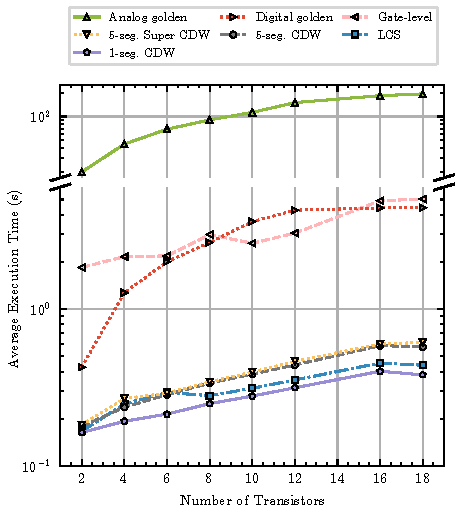
\includegraphics[width=0.48\textwidth,trim={0 1mm 0 1mm},clip]{images/ch2/execution_time_report_plot.pdf}
    \caption{Mean execution time for each approach plotted against the number of transistors for the circuit gates. Segment is abbreviated as seg.}
    \label{fig:Execution time}
\end{figure}

\subsection{Accuracy of Aging-Induced Degradation}
On the other hand, the accuracy of each approach is shown in Fig. \ref{fig:Mean error}, where the mean threshold voltage degradation prediction of each transistor in the digital circuit is compared to the prediction made by the baseline \textit{Analog Golden} approach, which is assumed to be the most accurate. The threshold voltage degradations are obtained by computing eq. (\ref{Equation:MeanVt}) for the $\text{P}_{\text{occ}}$ resulting from each approach. W2 (with sleep period) is harder to compress and results into higher errors. The \textit{Gate-level} approach outperforms the digital approaches, which are hindered by the accuracy loss from the \textit{Activity Monitoring} step. The \textit{1-segment CDW} and \textit{5-segment Super CDW} have an error similar to the \textit{Digital Golden} approach. The \textit{5-segment CDW} approach is more error-prone due to the distortion required to extend each segment to EOL, specially for workload W2. This is explained by the shape of the waveform in W2, where the last $\qty{2}{\micro s}$ are extended to 2 years following the original approach (see Fig. \ref{fig:CDWvsSuperCDW} again for a detailed example). Assuming that the circuit is under continuous operation for 8 years followed by 2 years in sleep is a completely different degradation scenario than having a circuit which operates for $\qty{8}{\micro s}$ followed by $\qty{2}{\micro s}$ sleep continuously. The 2 years of sleep mode are essentially 2 years of DC stress, with conducting transistors capturing many carriers and non-conducting transistors releasing most of the captured ones. This issue does not exist with the \textit{Super CDW} approach, as the EOL extrapolation is correctly made without modifying the length of each segment and distorting the signal. Finally, the \textit{LCS} approach has a significant error under both scenarios because it fails to predict the long-term \gls{BTI} caused by complex waveforms. Using two long DC periods to model long-term stress will result in a different set of defects being captured when compared to a complex waveform with quick successions of stress and recovery. 
\begin{figure}[!t]
    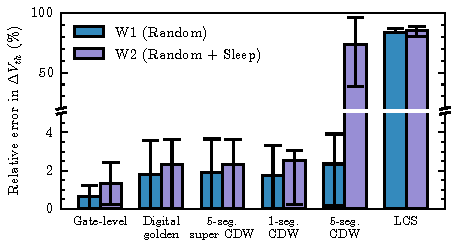
\includegraphics[width=0.48\textwidth,trim={0 1mm 0 0},clip]{images/ch2/mean_error_bar_scatter_report_plot.pdf}
    \caption{Mean relative error with error bars for 10th-quantiles and 90th-quantiles of the considered approaches when predicting the threshold voltage degradation of each transistor after comparing the prediction to the golden analog reference for both workloads under consideration. Transistors with a duty cycle of 0 or 1 are not considered as DC stress requires no compression. }
    \label{fig:Mean error}
\end{figure}
Given how the W2 workload is the hardest to compress accurately for all approaches, it will be the one used moving forward. A closer look into the error in predicting the degradation of each transistor is shown in Fig. \ref{fig:cellwise error}. These results confirm how \textit{Activity Monitoring} is causing the errors for the \textit{Digital Golden} approach in complex cells (those errors above 10 mV) that are harder to translate from input signal to transistor duty cycle, as discussed in subsection \ref{ss:ExtendingCASE}. Meanwhile, transistors corresponding to inverters (i.e., those within a 2-transistor gate) do not have a significant error for the \textit{Digital Golden} approach. The \textit{Activity Monitoring} errors are carried into the \textit{1-segment CDW} and \textit{5-segment Super CDW} predictions, as they employ a digital format for the workload. It is also clear how the \textit{LCS} and \textit{5-segment CDW} approaches fail to accurately represent the degradation of most transistors.

\begin{figure}[!t]
    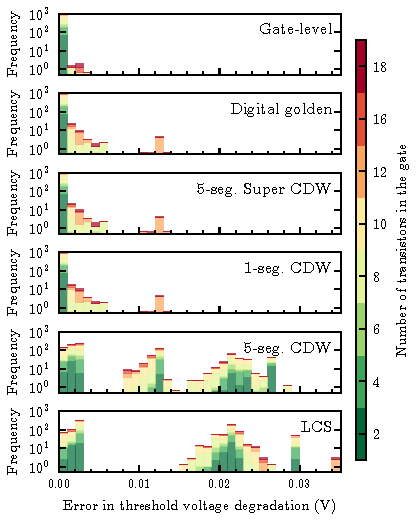
\includegraphics[width=0.48\textwidth,trim={0 0 0 1mm},clip]{images/ch2/absolute_error_histogram_plot.pdf}
    \caption{Error in threshold voltage degradation prediction for each transistor in the circuit using workload W2. The transistors are differentiated depending on the complexity (defined as the number of transistors) of their corresponding gate.}
    \label{fig:cellwise error}
\end{figure}

%In any case, if short-term \gls{BTI} is a concern, one may add a LCS phase to any of the previous approaches without a significant cost in execution time. 

    % The large error bars are mostly due to outliers caused by transistors with a duty cycle close to 0 or 1, where a small difference in the waveform can result in a large relative difference in degradation.
\subsection{Delay change estimation}

It is important to translate the threshold voltage degradation, which is a transistor-level parameter, into the relevant circuit-level figure of merit for digital standard cells, i.e., propagation delays. A detailed list of the logic gates present in the 32-bit MAC design is shown in Table \ref{table:gates}, ranging in complexity from 2-transistor inverters to 18-transistor 8-input complex cells such as AOI332. A digital gate with more than one input will have more than one valid timing path for a transition propagating from input to output. A change in the output with a certain unateness requires the appropriate, gate-dependent combination of input values (determined by the logic operation of the gate), and the propagation delay will be different depending on the timing path's input and the state of the other inputs. In this way, the number of possible delays increases rapidly with the number of gate inputs, as shown in the second column of Table \ref{table:gates}. 

\begin{table}
	\caption{32-bit MAC gates and their characteristics}
	\begin{center}
		\begin{tabular}{lcccc} \toprule
			Gate & Inputs & Delay combinations & Transistors & Instances \\ \midrule
			INV & 1 & 2 & 2 & 103 \\
			NOR2 & 2 & 4 & 4 & 25 \\
			NAND2 & 2 & 4 & 4 & 62 \\
			XOR2 & 2 & 8 & 10 & 48 \\
			XNOR2 & 2 & 8 & 10 & 66 \\
			NAND3 & 3 & 6 & 6 & 25 \\
			OAI21 & 3 & 10 & 6 & 7 \\
			AOI21 & 3 & 10 & 6 & 4 \\
			AO21 & 3 & 10 & 8 & 2 \\
			NOR4 & 4 & 8 & 8 & 2 \\
			NAND4 & 4 & 8 & 8 & 4 \\
			AND4 & 4 & 8 & 10 & 2 \\
			OAI211 & 4 & 16 & 8 & 1 \\
			A2O1A1I & 4 & 20 & 8 & 40 \\
			OAI31 & 4 & 20 & 8 & 2 \\
			AOI31 & 4 & 20 & 8 & 2 \\
			AOI22 & 4 & 24 & 8 & 8 \\
			OAI22 & 4 & 24 & 8 & 20 \\
			OAI222 & 6 & 108 & 12 & 16 \\
			AOI332 & 8 & 448 & 16 & 13 \\
			OAI332 & 8 & 448 & 16 & 2 \\
			AO332 & 8 & 448 & 18 & 3 \\
			OA332 & 8 & 448 & 18 & 2 \\ \bottomrule
		\end{tabular}
	\end{center}
	\label{table:gates}
\end{table}


\begin{figure}[!t]
    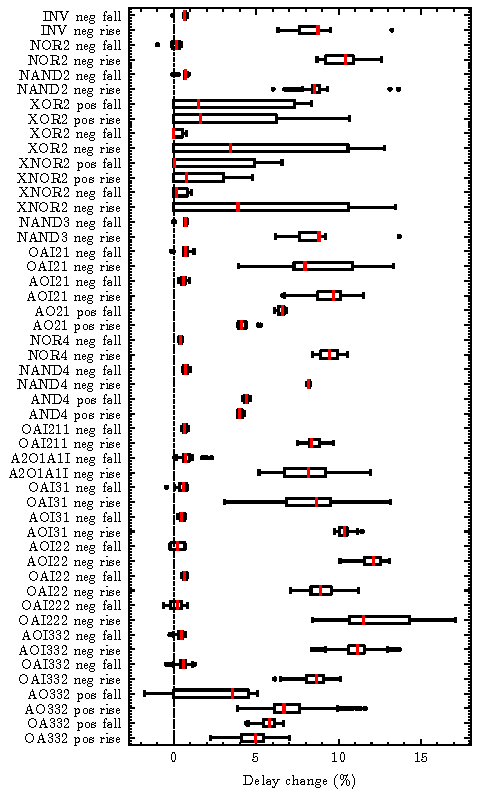
\includegraphics[width=0.48\textwidth,trim={0 0 0 0},clip]{images/ch2/box_cellwise_delay.pdf}
    \caption{Box plot showing the distribution of the mean increases in delay caused by aging degradation, using the \textit{Analog Golden} approach and the W2 workload. }
    \label{fig:cellwisedelay}
\end{figure}

With these considerations in mind, the delay change distributions are shown in Fig. \ref{fig:cellwisedelay}. A distinction is made between rise and fall delays as well as their unateness, which may be positive (0 $\xrightarrow{}$ 1, ``pos'') or negative (1 $\xrightarrow{}$ 0, ``neg''). Not all combinations are possible for all gates by construction. There are also edge cases where only the transistors that oppose the change in output value when a transition occurs are the ones that degrade, resulting in a delay reduction, which explains the small negative values \cite{santana-andreoImpactBTIHCI2022}. Beyond the gate characteristics, degradation is driven, naturally, by the workload that propagates from the MAC inputs to each individual gate. The variety in distributions for each gate in Fig. \ref{fig:cellwisedelay} clearly illustrates why careful and precise transistor-level predictions of degradation are necessary to arrive at the delay increase of each gate. These distributions are for the mean degradation, and the aging variability of each transistor needs to be considered on top of it to obtain a complete aging prediction. 

%An important factor to consider is the fact that \gls{BTI} degradation in PMOS (Negative Bias Temperature Instability, NBTI) is significantly greater than \gls{BTI} degradation in NMOS (Positive Bias Temperature Instability, PBTI). This can be clearly distinguished in the aforementioned topologically simpler gates (INV, NAND, NOR ...) where the increase in rise delay, determined mostly by the degradation of the pull-up network (NBTI), is significantly larger than the increase in fall delay, determined mostly by the degradation of the pull-down network (PBTI).

Given these degradation values in terms of the delay obtained for the \textit{Analog Golden} workload, they can be compared to the degradation obtained through each compression method. The resulting error is expressed in terms of percentage points (p.p.). To clarify with an example, given a delay increase of 10\%, if the prediction of the compressed waveform results in an increase of 6\% the error is $-4$ p.p. (40\% less), while if the prediction is of 12\% the error is $2$ p.p. (20\% more). An overestimation (positive p.p.) implies that the gate will not degrade as much as predicted, leading to design overcompensation when specifying the guardband and just an unnecessary performance loss. Meanwhile, an underestimation (negative p.p.) implies that the gate will degrade more than expected, leading to unacceptable timing violations. Hence, slight overestimation is fine, while even minor underestimation is catastrophic. The compression errors are shown in detail in Fig. \ref{fig:delay_compression_error}. The \textit{Gate Level} approach manages the best accuracy, matching the original degradation in most cases. \textit{Digital Golden}, \textit{1-segment CDW} and \textit{5-segment Super CDW} are similar in accuracy, having a higher error than the previous approach, with the \textit{1-segment CDW} method having a slightly larger number of overestimations.  All four of these distributions are reasonably symmetric, not exceeding 3 p.p. of over- or underestimation in any case. The \textit{5-segment CDW} does introduce significant errors in both directions, ranging from $-10$ p.p. of underestimation and 7.5 p.p. of overestimation. Given how the highest degradations observed in Fig. \ref{fig:cellwisedelay} are around 12.5\%, these errors are large. The \textit{LCS} method leads almost exclusively into underestimation, due to the inability to capture long-term degradation by applying the recovery phase. 

\begin{figure}[!t]
    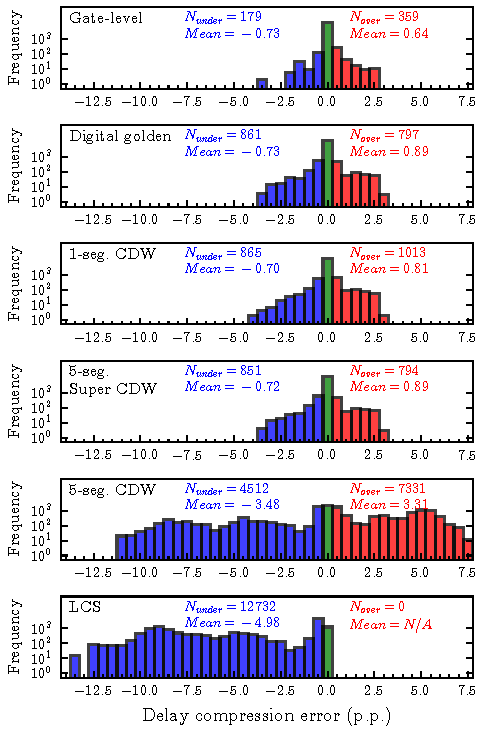
\includegraphics[width=0.48\textwidth,trim={0 0 0 0},clip]{images/ch2/error_delay_report_plot.pdf}
    \caption{Distributions for errors in the delay estimation of each compression method expressed in percentage points for workload W2. Mind the logarithmic scale for the y-axis. Underestimations, which can lead to timing violations, are shown in blue, while overestimations, which can lead to unnecessary performance loses, are shown in red. Those cases where compression matches the original prediction are shown in green.}
    \label{fig:delay_compression_error}
\end{figure}

\subsection{Frequency dependence}
\label{subsection:freq_dependence}
The technique detailed in subsection \ref{subsection:Defect_distribution_shifting} is employed to analyze the performance of each compression method under different frequency scenarios. The short-term component of \gls{BTI} is driven by the latest bias conditions of the transistor. In low-frequency scenarios, the time transistors are at a high or low bias before switching increases, making the short-term component greater in amplitude, as stress and relaxation times are longer. The time constants are shifted by a certain \textit{frequency factor} (without any loss in accuracy, see subsection \ref{subsection:Defect_distribution_shifting}), which determines the shift in terms of orders of magnitude. For example, applying a \textit{frequency factor} of 3, $f_\text{clk}$ goes from $\qty{100}{MHz}$ to $\qty{100}{kHz}$ and the workload duration goes from $\qty{10}{\micro s}$ to $\qty{10}{ms}$. Frequency factors range from $-1$ to 9, to get a wide range of frequencies from GHzs to $<$ 1 Hz. To evaluate the performance of each compression method, the number of overestimations, underestimations, and mean deviation for each case are used, as in Fig. \ref{fig:delay_compression_error}. 

\begin{figure}[!t]
    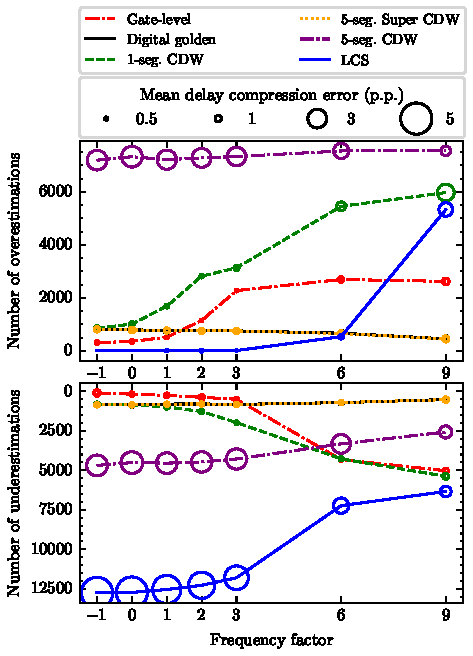
\includegraphics[width=0.48\textwidth,trim={0 0 0 0},clip]{images/ch2/delay_error_frequency_dependence.pdf}
    \caption{Bubble chart indicating the number of over and under estimations in terms of delay prediction from each compression method for a set of different \textit{frequency factors} and workload W2. The bubble size indicates the mean deviation. The \textit{Digital Golden} and \textit{5-segment Super CDW} approaches overlap each other in accuracy.}
    \label{fig:delay_error_frequency_dependence}
\end{figure}
\begin{figure}[!t]
    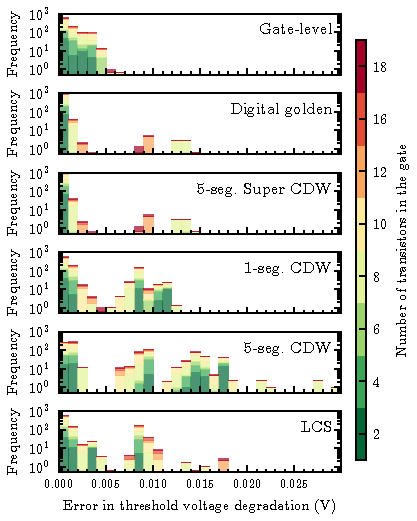
\includegraphics[width=0.46\textwidth,trim={0 0 0 1mm},clip]{images/ch2/absolute_error_histogram_plot_tau6.pdf}
    \caption{Error in threshold voltage degradation prediction for each transistor in the circuit, workload W2 and a \textit{frequency factor} of 6.}
    \label{fig:cellwise error tau6}
\end{figure}
The results are shown in Fig. \ref{fig:delay_error_frequency_dependence}. It is clear that the conclusions extracted from the original workload do not hold for the entire frequency range. \textit{Digital Golden} and \textit{5-segment Super CDW} are able to maintain a consistent error rate, associated with the \textit{Activity Monitoring} step, and which slightly decreases with slower frequency as the importance of that error is reduced when the short-term component becomes stronger. It is remarkable to note that the \textit{5-segment Super CDW} compression is able to exactly match the \textit{Digital Golden} accuracy. Both the \textit{Gate-level} and \textit{1-segment CDW} suffer from the fact that they cannot properly represent the heterogeneity of the signal. Although for high frequencies \textit{Gate-level} is the best in terms of accuracy and \textit{1-segment CDW} matches \textit{Digital Golden} and \textit{5-segment Super CDW}, they start to become inaccurate (over- and underestimations, higher mean error) when frequency decreases. For the \textit{1-segment CDW} this is consistent with the results shown in Fig. \ref{fig:CDWTestFinishSweep} (b) and discussed in Subsection \ref{subsection:SuperCDWcompression}: Increasing the number of CDW segments and correctly representing the heterogeneity of the signal becomes more important as the short-term component of \gls{BTI} becomes more significant. The \textit{Gate-level} generates a synthetic workload that matches the characteristics of the entire representative workload but is not able to capture the hetereogenity of the signal to model the short-term component properly. Finally, both \textit{5-segment CDW} and \textit{LCS} are not able to accurately represent the degradation for the entire range. These conclusions are further supported by inspecting the error in the threshold voltage degradation for a specific \textit{frequency factor}, as shown in Fig. \ref{fig:cellwise error tau6} for a \textit{frequency factor} of 6. \textit{5-segment Super CDW} and \textit{Digital Golden} have the error associated with \textit{Activity Monitoring} and complex cells, while \textit{Gate-level} and \textit{1-segment CDW} perform significantly worse than with the original frequency. \textit{LCS} performs better when short-term \gls{BTI} is more dominant, it shifts from underestimation to overestimation as the longest continuous stress time increases at lower frequencies. Overestimation is a built-in feature of \textit{LCS} as it tries to provide the worst-case degradation scenario. It is clear how, when considering which compression method to employ, the frequency of the signal is important. Given that there is no universal switching frequency for a large digital circuit, it is not straightforward to have a clear cut-off point for all instances in the circuit. In that context, the \textit{5-segment Super CDW} is clearly superior and the best general approach given the aforementioned variety in switching frequencies, as it achieves great accuracy and low execution times across the board. However, considering that originally the input signal changes every 10 ns with a $f_\text{clk}$ of 100 MHz and that both the \textit{Gate-level} and \textit{1-segment CDW} approaches become comparatively worse to the \textit{5-segment Super CDW} for a \textit{frequency factor} of 2, we can estimate that, in this specific scenario, for a $f_\text{clk}$ in a range of GHzs to tens of MHzs, using the \textit{Gate-level approach} is best for accuracy, and using a \textit{1-segment CDW} is valid for speed. 





\section{Conclusions}
\label{section:Conclusions}

After a thorough exploration of the compression techniques found in the literature and comparing them on the same workload and circuits for the first time, we have successfully introduced two novel approaches (\textit{Gate-level} and \textit{Super CDW} compression) that surpass existing methods in terms of speed and accuracy. The accuracy of each compression method is not solely evaluated based on the predicted threshold voltage shift per transistor, but additionally also wholistically, i.e., with aging-aware circuit delay estimations. We explored a wide range of conditions (e.g., switching frequencies) to illustrate the robustness of our proposed techniques. For the entire range of frequency values, using the compression methods found in the literature (\textit{CDW} and \textit{LCS}) yields unacceptable results (up to 73.34\% for the \textit{5-segment CDW} average error in threshold voltage and 84.85\% for \textit{LCS}) in terms of accuracy. On the other hand, the proposed \textit{Super CDW} method performs well in the entire frequency range in terms of accuracy and speed. Specifically, it is 295X faster compared to the analog uncompressed workload, 8X faster than the digital uncompressed workload, and has a 2.31\% average error in threshold voltage degradation, matching the digital uncompressed workload, while featuring a low upper bound for execution time and making it the superior choice in most scenarios. For high transistor switching frequencies, \textit{Gate-level} is the best choice in terms of accuracy (1.31\% average error in threshold voltage degradation) and \textit{1-segment CDW} is the best choice in terms of speed (1.27X faster than \textit{5-segment Super CDW)}, but both drop significantly in accuracy as frequency decreases. Hence, only the proposed \textit{Super CDW} technique with an appropriate number of segments has a consistent, low error rate for the entire range of switching frequencies.

%due to their inability to correctly represent the impact of a workload's heterogeneity on the short-term component of BTI.

% In future work, these approaches will be used to predict the long-term degradation of larger digital circuits with a strong foundation in the physics of \gls{BTI} without compromising speed. 
